\documentclass[12pt]{article}
\setlength{\oddsidemargin}{0in}
\setlength{\evensidemargin}{0in}
\setlength{\textwidth}{6.5in}
\setlength{\parindent}{0in}
\setlength{\parskip}{\baselineskip}
\usepackage{amsmath,amsfonts,amssymb}
\usepackage{graphicx}
\usepackage{enumitem}
\usepackage[]{algorithmicx}
\usepackage{amsthm}
\usepackage{fancyhdr}
\pagestyle{fancy}
\setlength{\headsep}{36pt}
\usepackage{tkz-berge}
\usetikzlibrary{positioning, automata}

\usepackage{hyperref}

\theoremstyle{remark}
\newtheorem*{solution}{Solution}

\newcommand{\makenonemptybox}[2]{%
%\par\nobreak\vspace{\ht\strutbox}\noindent
\item[]
\fbox{% added -2\fboxrule to specified width to avoid overfull hboxes
% and removed the -2\fboxsep from height specification (image not updated)
% because in MWE 2cm is should be height of contents excluding sep and frame
\parbox[c][#1][t]{\dimexpr\linewidth-2\fboxsep-2\fboxrule}{
  \hrule width \hsize height 0pt
  #2
 }%
}%
\par\vspace{\ht\strutbox}
}
\makeatother

\begin{document}
\definecolor {processblue}{cmyk}{0.96,0,0,0}

\lhead{{\bf CSCI 3104, Algorithms \\ Problem Set 4b (45 points)} }
\rhead{Name: Luna McBride \\ ID: 107607144 \\ {\bf Profs.\ Hoenigman \& Agrawal\\ Fall 2019, CU-Boulder}}
\renewcommand{\headrulewidth}{0.5pt}

\phantom{Test}

\begin{small}
\textbf{Instructions for submitting your solution}:
\vspace{-5mm} 

\begin{itemize}
	\item The solutions \textbf{should be typed} and we cannot accept hand-written solutions. \href{http://ece.uprm.edu/~caceros/latex/introduction.pdf}{Here's a short intro to Latex.}
	\item You should submit your work through \href{https://www.gradescope.com/courses/59294}{\textbf{Gradescope}} only.
	\item If you don't have an account on it, sign up for one using your CU email. You should have gotten an email to sign up. If your name based CU email doesn't work, try the identikey@colorado.edu version. 
	\item Gradescope will only accept \textbf{.pdf} files (except for code files that should be submitted separately on Gradescope if a problem set has them) and \textbf{try to fit your work in the box provided}. 
	\item You cannot submit a pdf which has less pages than what we provided you as Gradescope won't allow it. 
	\item Verbal reasoning is typically insufficient for full credit. Instead, write a logical argument, in the style of a mathematical proof.
	\item For every problem in this class, you must justify your answer:\ show how you arrived at it and why it is correct. If there are assumptions you need to make along the way, state those clearly.
	
	\item You may work with other students. However, \textbf{all solutions must be written independently and in your own words.} Referencing solutions of any sort is strictly prohibited. You must explicitly cite any sources, as well as any collaborators. 
\end{itemize}



\vspace{-4mm} 
\end{small}

\hrulefill

\newpage
\begin{enumerate}

\item (10 pts) For a directed graph with positive weights, we define the max-weight of a path from $s$ to $d$ as the maximum of the edge weights along the path. For example, if the path from A to D has edges and weights of $e_{AB} = 5$, $e_{BC} = 4$, and $e_{CD}=1$, the length of the path is defined as $e_{AB} + e_{BC} + e_{CD}$, and the max-weight is 5.
\begin{enumerate}
\item(5 pts) Give an algorithm to compute the smallest max-weight paths from a source vertex s to all other vertices. In this problem, you are changing the definition of length of the path from A to D to $max(e_{AB}, e_{BC}, e_{CD})$ (Hint: Your algorithm should be a modification of Dijkstra's algorithm presented in Lecture.)

\begin{solution}
$\newline$ ModDijkstra(G,S): $\newline -$  max=0 $\newline -$ Initialize dist, prev for all vertices plus max edge weight  $\newline -->$ dist(s)=0  $\newline -->$ dist(v)=$\infty$   $\newline -->$ Q=min priority queue  $\newline -->$ Q.add(v)   $\newline --$ while Q!empty:  $\newline ----/$  u=Q.pop() $\newline ----/$ for each vert in u,adjacent: $\newline ----/-->$d=dist(v)+edge(u,v) $\newline ----/-->$ if d$<$dist(v): $\newline ----/--/-->$ dist(v)=d $\newline ----/--/-->$ prev(v)=u $\newline \newline --$ for i in range 0, len(vertices): $\newline ----/$ d=dist(v[i]) $\newline ----/$ if max $<$ d:  $\newline ----/-->$ max=d $\newline -$ return G
\end{solution}

\pagebreak
\item(5 pts) Prove the correctness of your algorithm.
\end{enumerate}
\begin{solution}
$\newline$ Loop Invariance for the added for loop: dist(v[0]), dist(v[1])...dist(v[i-1]) $\leq$ max for the already completed version of Dijkstra's algorithm. $\newline \newline$ Base case: dist(v[0]) is greater than 0, which max is then set equal to. max is then equal to the only vertex checked, which fits into the $\geq$ title. $\newline \newline$ Maintanence: For every iteration of the loop, max is set to the biggest value it comes across. Any value less than the current max can then be ignored, as it is not the max. Thus, as the largest value is contained in max, which means every value dist(v[0-(i-1)]) is necessarily less than or equal to max. $\newline \newline$ Termination: On the last iteration, the max either keeps the last value if it is the largest or ignores it because it is less than the current max. In either case, the largest value overall is now contained within the max variable. This means that every single distance value for every vertex is either less than or equal to max. $\newline \newline$ Since the shortest path has already been obtained before this invariance relation comes into play and it does obtain the maximum as shown in the invariance, then the max value is the maximum value needed within the shortest path.
\end{solution}

\pagebreak

\item (11 pts) Based on the following graph :
\begin{figure}[h!]
\begin{center}
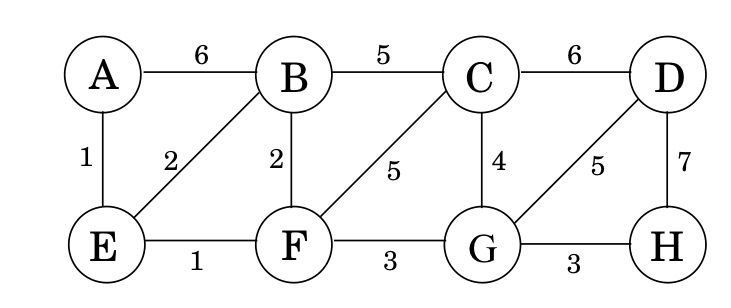
\includegraphics[scale=0.3]{mst_graph_q2.jpg} 
\end{center}
\end{figure}

\begin{enumerate}[label=(\alph*)]

\item (4 pts) In what order would Prim's algorithm add edges to the MST if we start at vertex $A$? 
\begin{solution}
$\newline \pagebreak$ $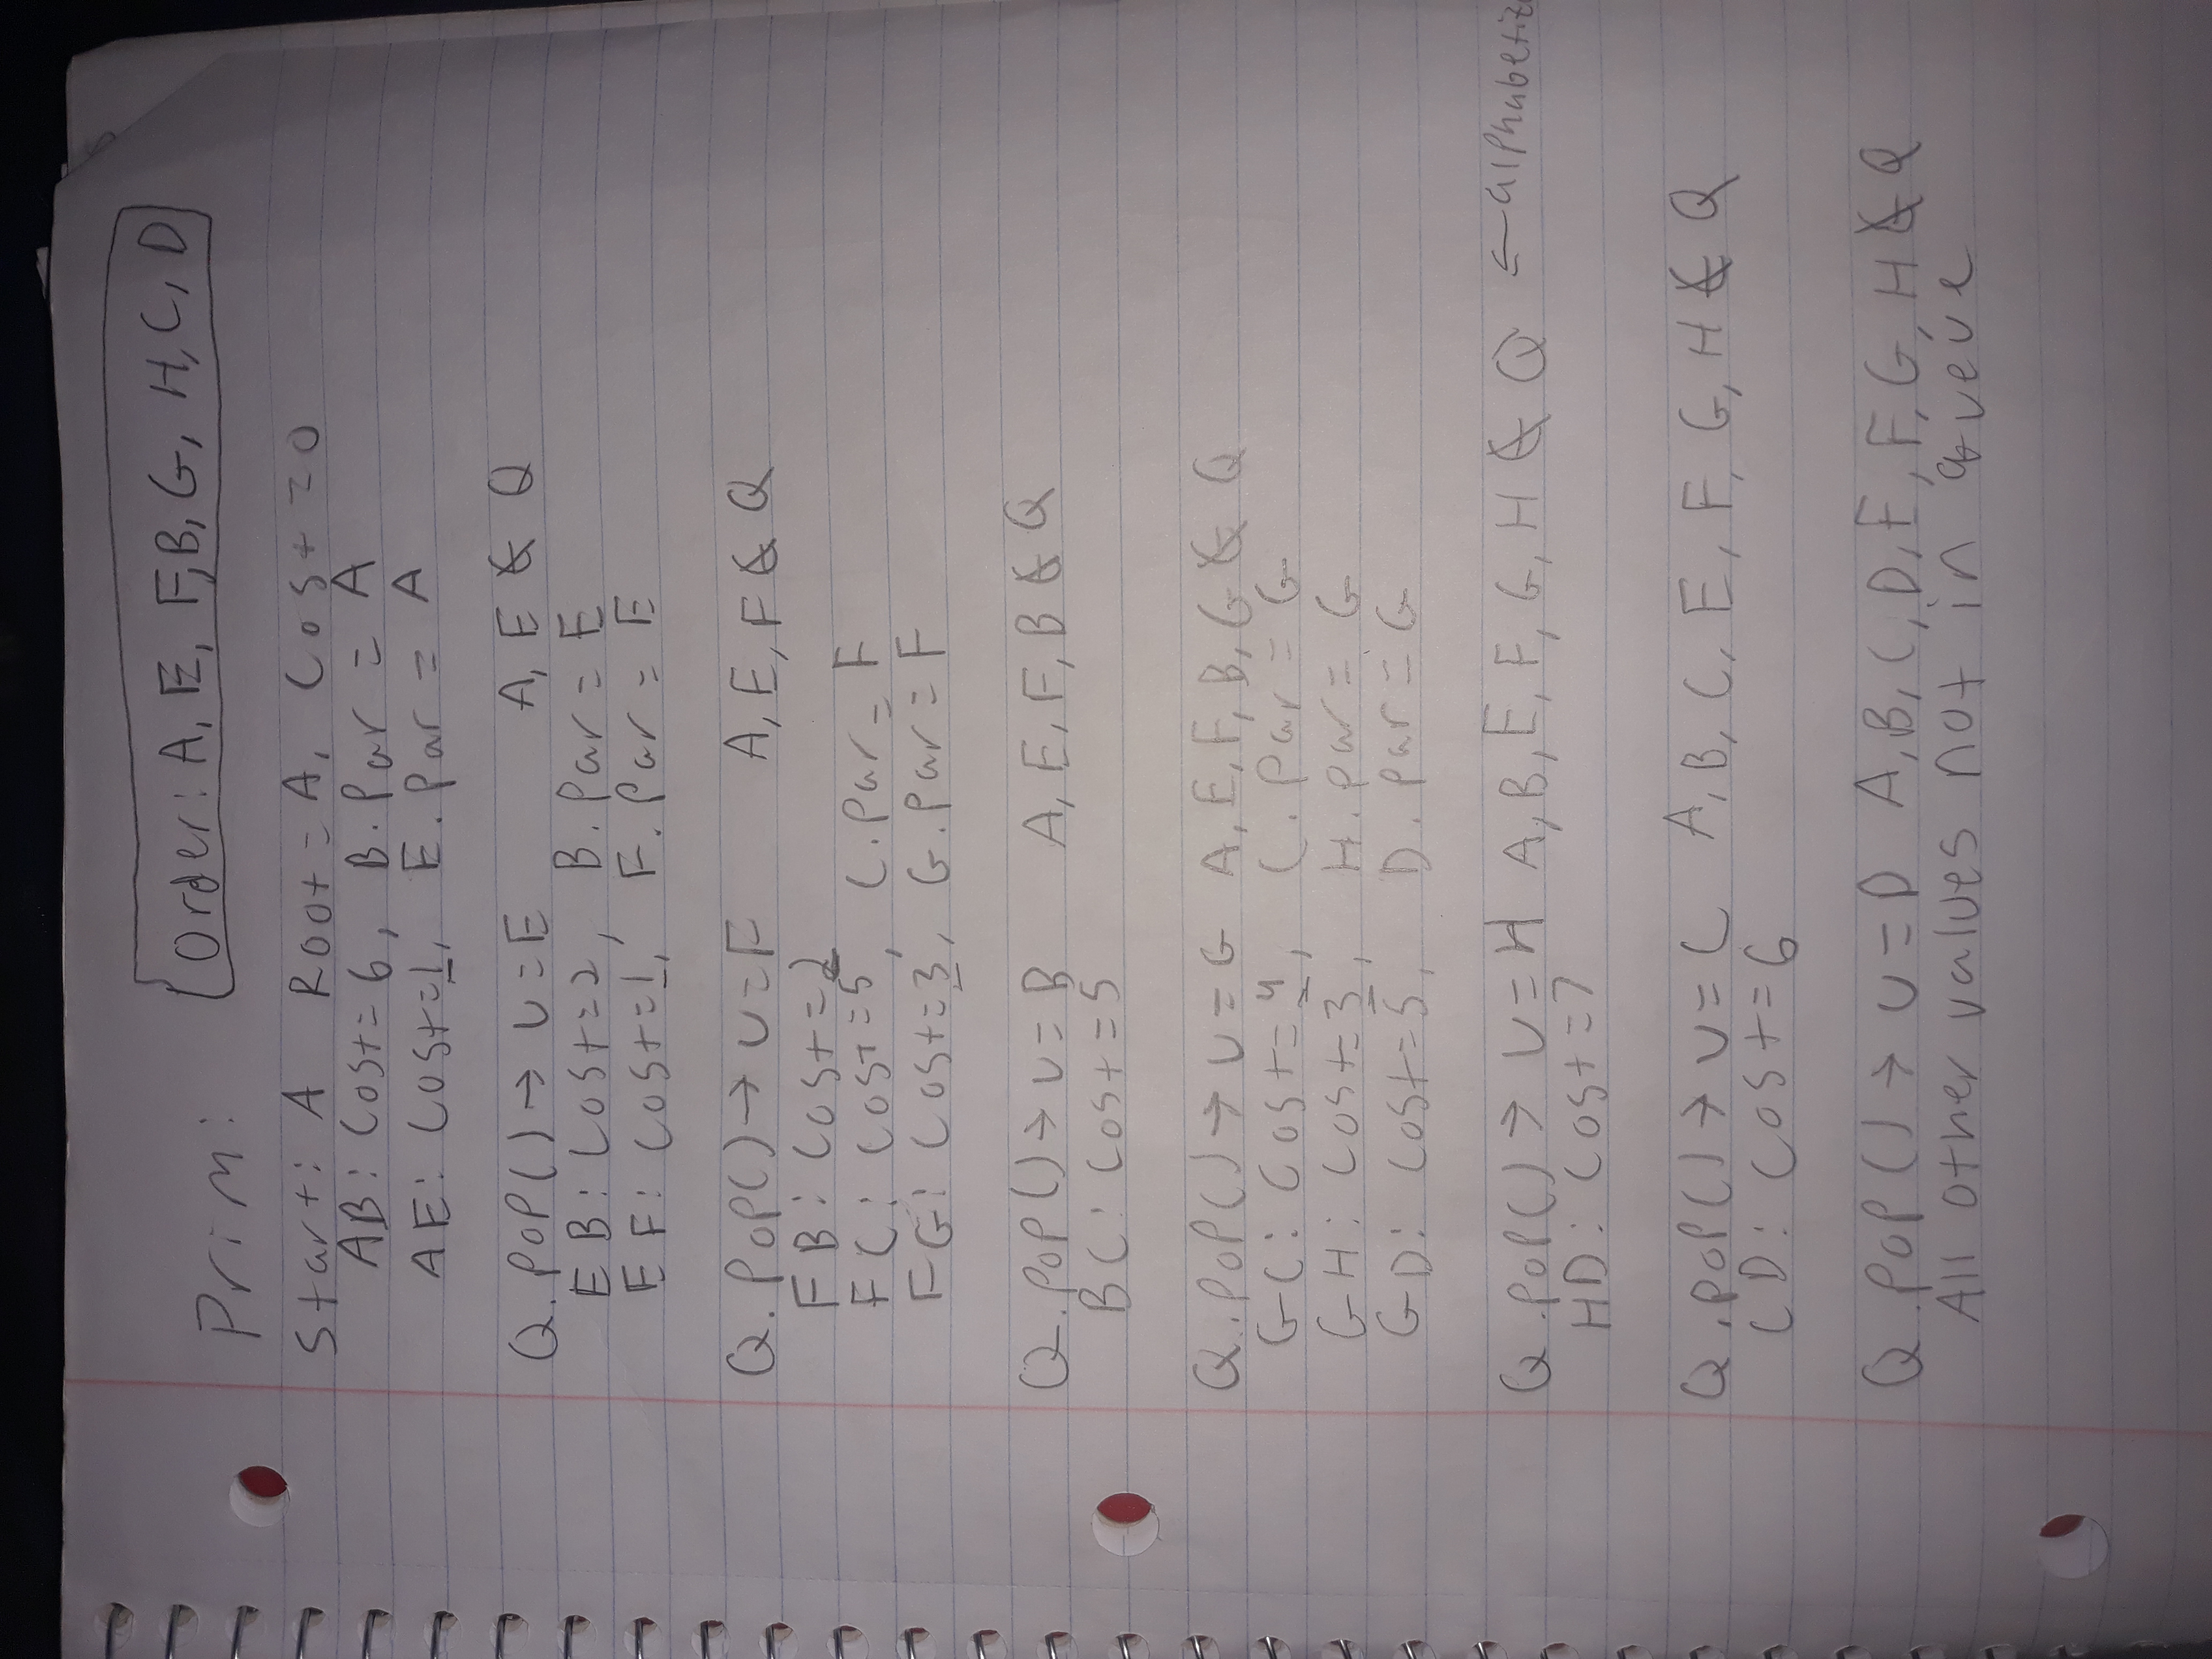
\includegraphics[width=7.7in, height=6in, angle=-90]{Prim}$
\end{solution}
\pagebreak
\item (7 pts) In what order Kruskal's would add the edges to the MST? For each edge added by Kruskal's sequentially, give a cut that justifies it's addition. 
\begin{solution}
$\newline$ From left to right (following value assention): $\newline \newline$ For A: p1={A}, p2={B,C,D,E,F,G,H}. Edges in cut: AB=6, AE=1. 6$>$1, so AE is chosen. $\newline \newline$ p1={E}, p2={A,B,C,D,F,G,H}. AE is already chosen, so Edges in cut: EB=2, EF=1. 2$>$1, so EF is chosen. $\newline \newline$ Next: p1={A,B,C,D}, p2={E,F,G,H}.  Disregarding the already chosen AE, the smallest value in the cut is 2, both going to B. It could choose either (but not both), so I will go left to right and say EB=2 is chosen. $\newline \newline$ Next: p1={A,B,E,F}, p2={C,D,G,H}. The lowest in the cut is 3, so next chosen is FG=3. $\newline \newline$ Next: p1={A,B,C,E,F,G}, p2={D,H} (as there is a 3 in there). The value of 3 exists in this set, which is less than 5 and 6. Thus, GH=3 will be chosen $\newline \newline$Next: p1={A,B,C,D}, p2={E,F,G,H}. Previously looked at lines AE,EB,BF are ignored via cycles and already chosen values. The value CG is less than the other values in the set, so CG=4 is chosen. $\newline \newline$ Next: p1={D}, p2={A,B,C,E,F,G,H} (as it is the last node unconnected). The values here are 6,7,5. Since 5 is the lowest, GD=5 will be chosen. $\newline \newline$ All other edges will create loops, so the final edge list is [AE,EF,BE,FG,GH,CG,DG] at a weight of 19 (same ones listed above in the same order, but I put the edges in alphabetical order) 
\end{solution}
 

\end{enumerate}

\pagebreak

\item (10 pts) Let $T$ be a MST of a given graph $G$. Will $T$ still be the MST if we reduce the weight of exactly one of the edges in $G$ by a constant \textbf{c}? Prove your answer.
\begin{solution}
$\newline$ Well, let us say this assumption is true for any edge. Take a look at this image: $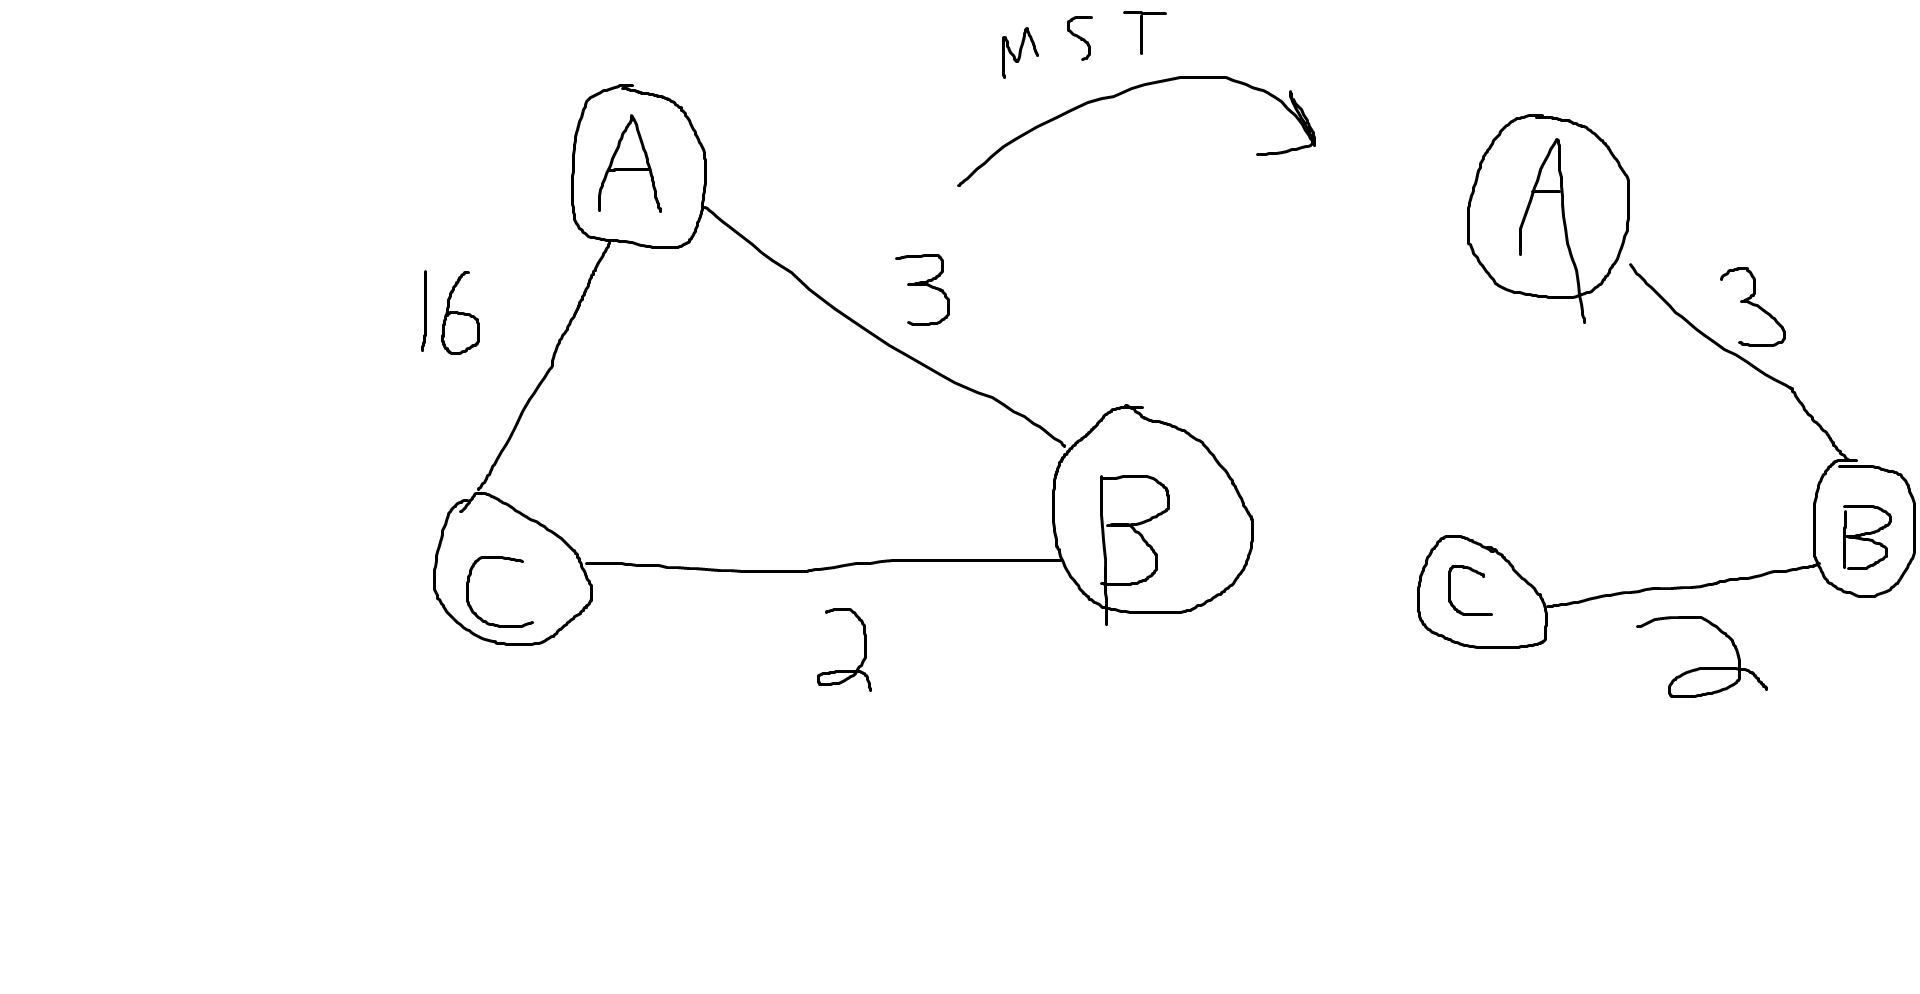
\includegraphics[scale=0.3]{TreeM} \newline$ This shows a basic graph and MST. For AB and BC, since these are already the required minimum, any lowering of them will not change the shape. Next, we have AC. $\newline \newline$ AC=16-c, AB=3, BC=2 $\newline \newline$ For the MST to stay an MST, for all c c$<$edgeweight (it must have a positive edge weight at all times), AC $\geq$ AB or BC, or 16-c $\geq$ 3 or 16-c $\geq$ 2, since otherwise this spanning tree is not the minimum by definition since there is a smaller edge. $\newline \newline$  Let us take AB as an example, since it is the largest between AB and BC $\newline \newline$ 16-c $\geq 3 --> 16 \geq 3+c --> 13 \geq c$ for AB to remain a minimum $\newline \newline$ However, 13 does not cover all possible c values. Since c$<$16, this leaves all values 13$<$c$<$16 that will create a smaller edge weight, which would turn that into an edge needed in the MST, negating the previous MST, putting it as just a spanning tree. $\newline \newline$ Therefore, by contradiction, T will not necessarily be a MST if we reduce one of the graph's edges by a constant c  $\newline 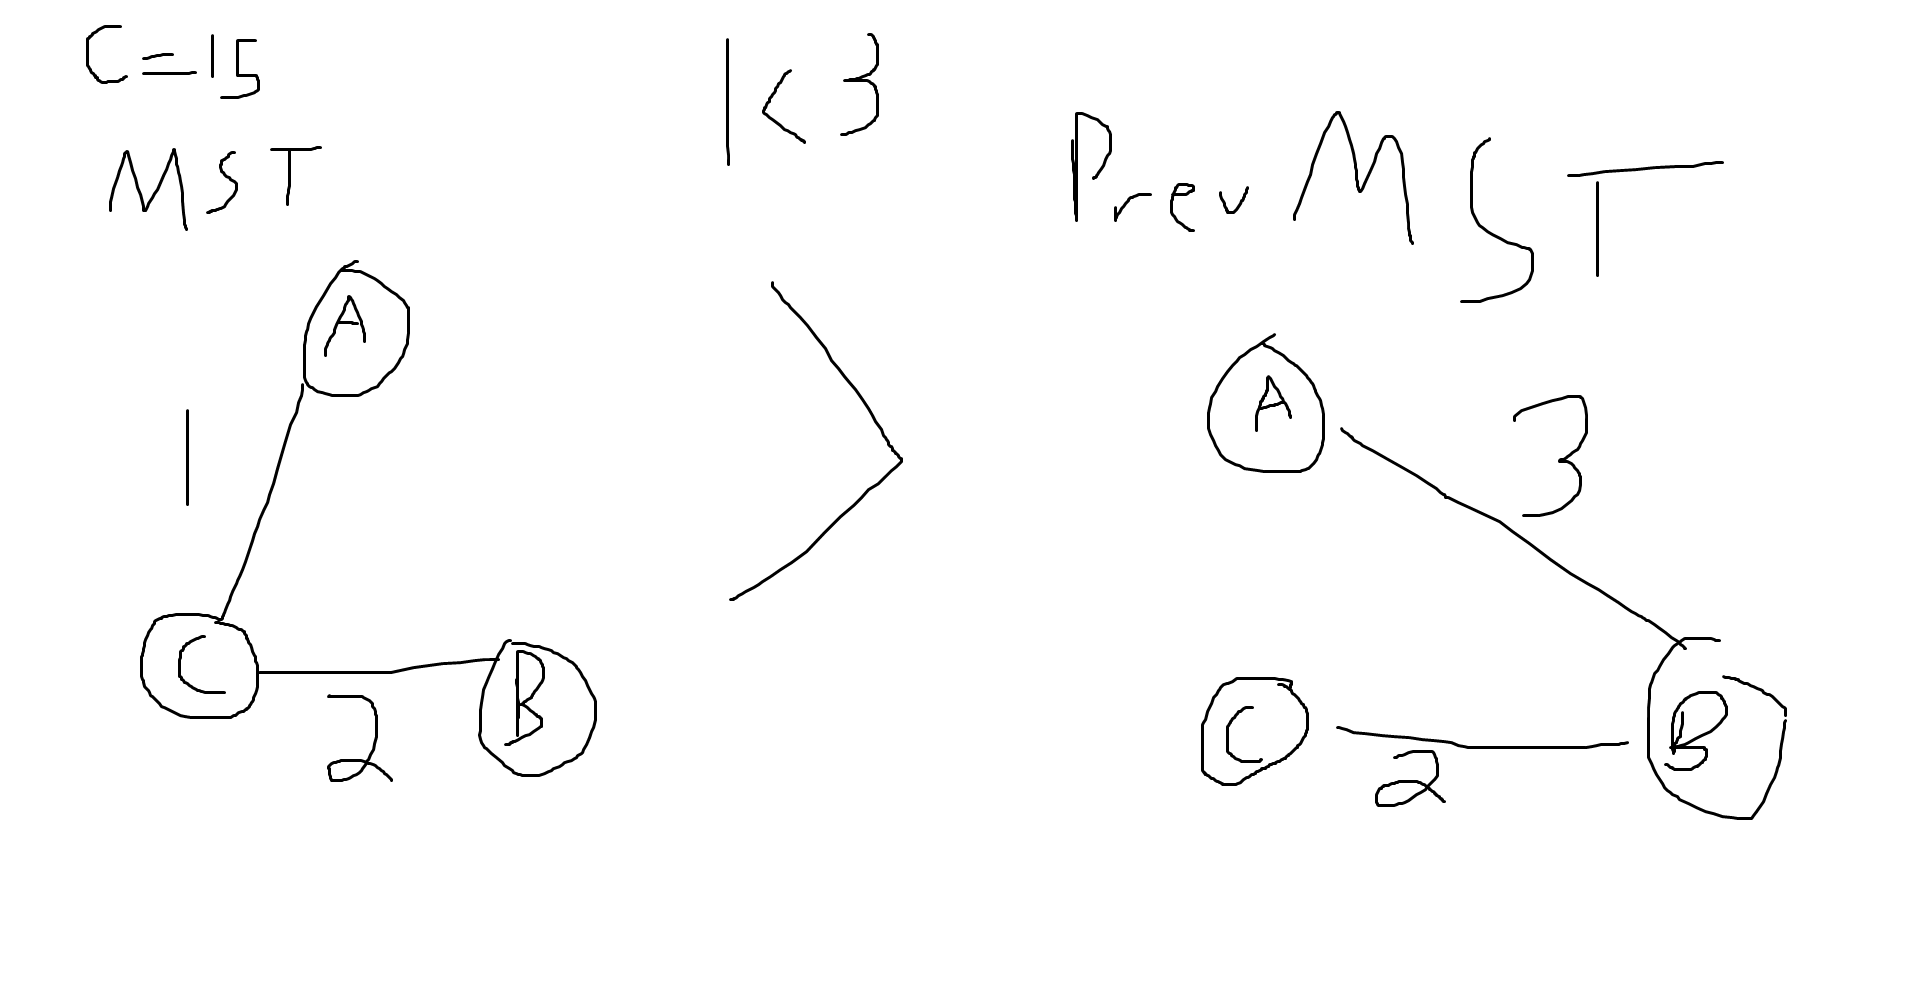
\includegraphics[scale=0.3]{TreeM2}$
\end{solution}

\pagebreak
\item (14 pts) One of the uses of MSTs is finding a set of edges that span a network for minimum cost. Network problems could also have another type of objective: designing a spanning tree for which the most expensive edge is minimized. Specifically, let $G = (V, E)$ be a connected graph with $n$ vertices, $m$ edges, and positive edge costs that you may assume are all distinct. Let $T = (V, E)$ be a spanning tree of $G$; we define the \textbf{limiting edge} of $T$ to be the edge of $T$ with the greatest cost.
A spanning tree $T$ of $G$ is a minimum-limiting spanning tree if there is no spanning tree $T$ of $G$ with a cheaper limiting edge.
\begin{enumerate}
\item (7 pts) Is every minimum-limiting tree of $G$ an MST of $G$? Prove or give a counterexample.
\begin{solution}
$\newline$ Assuming that all MLT are MST, Say we have this graph: $\newline$$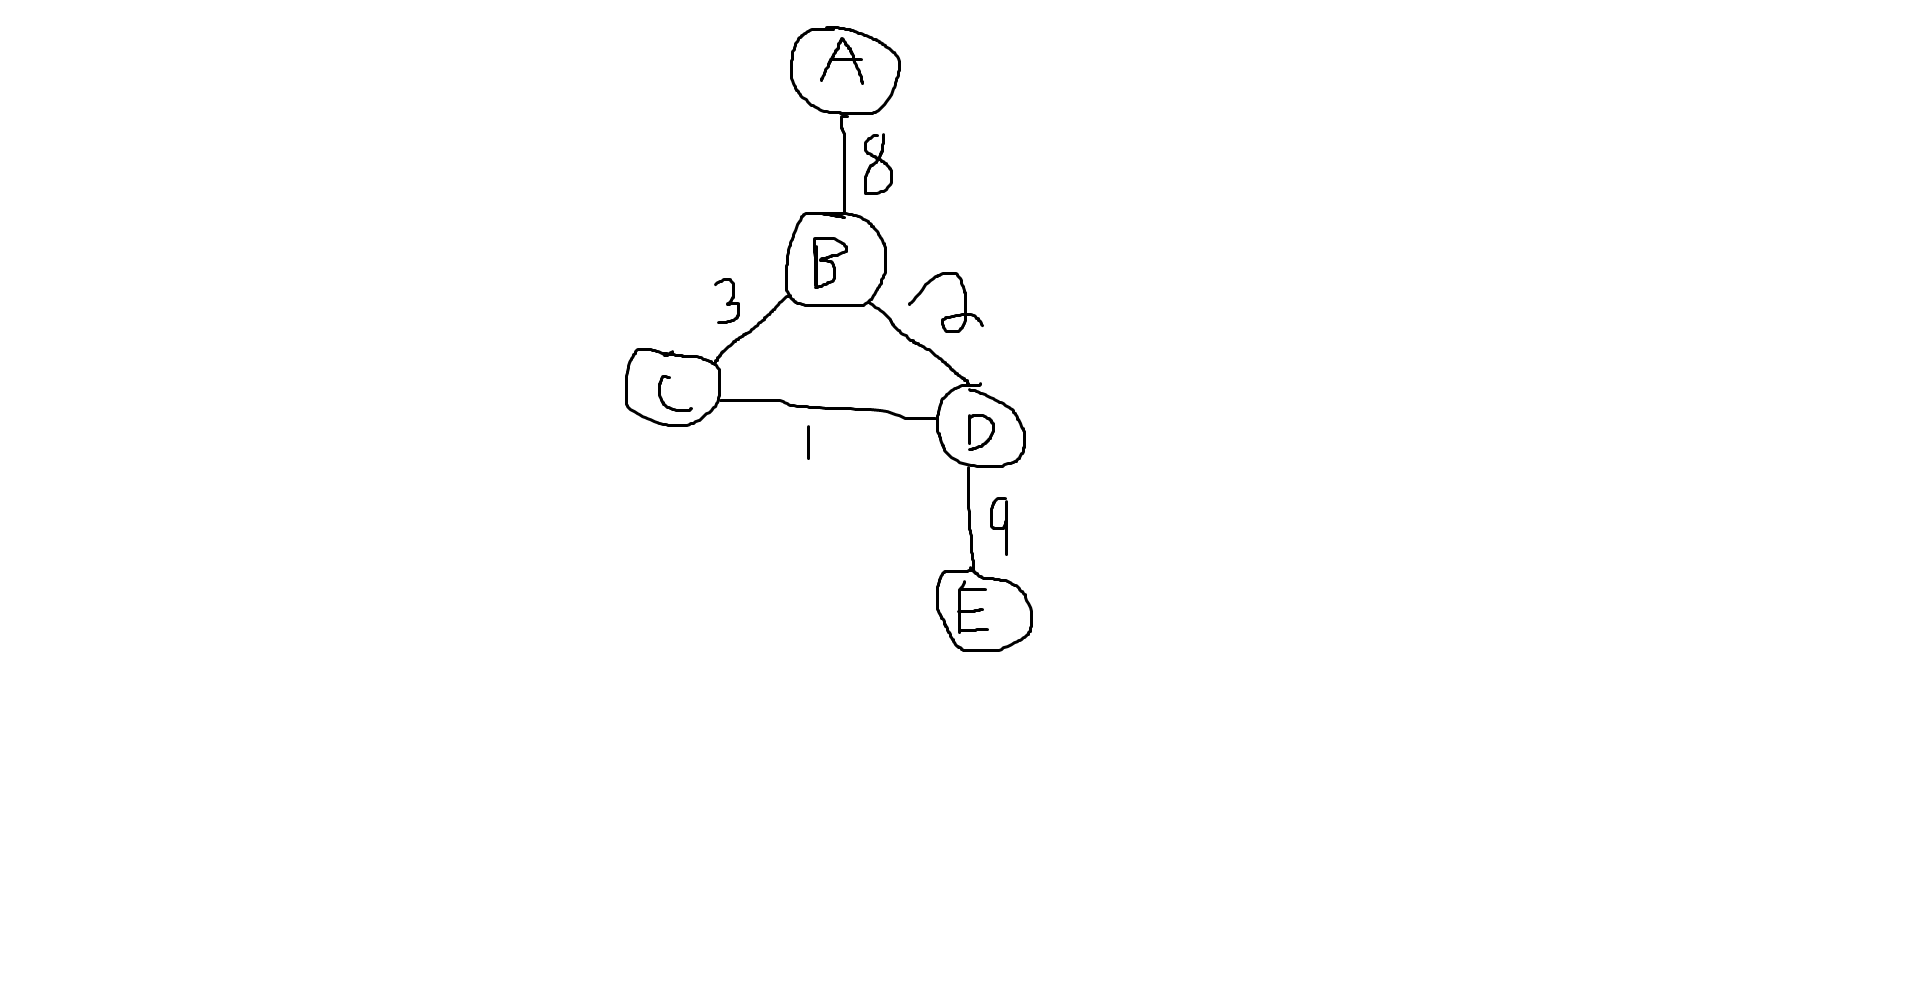
\includegraphics[scale=0.3]{MLT} \newline$ With this tree, edges DE and AB must necessarily be a part of all spanning trees, as otherwise, not all vertices are connected. That means the limiting edge is going to be DE, or 9, for every spanning tree, and thus every single spanning tree is also a limiting tree. $\newline \newline$ Taking this, we can look at this spanning tree:  $\newline$$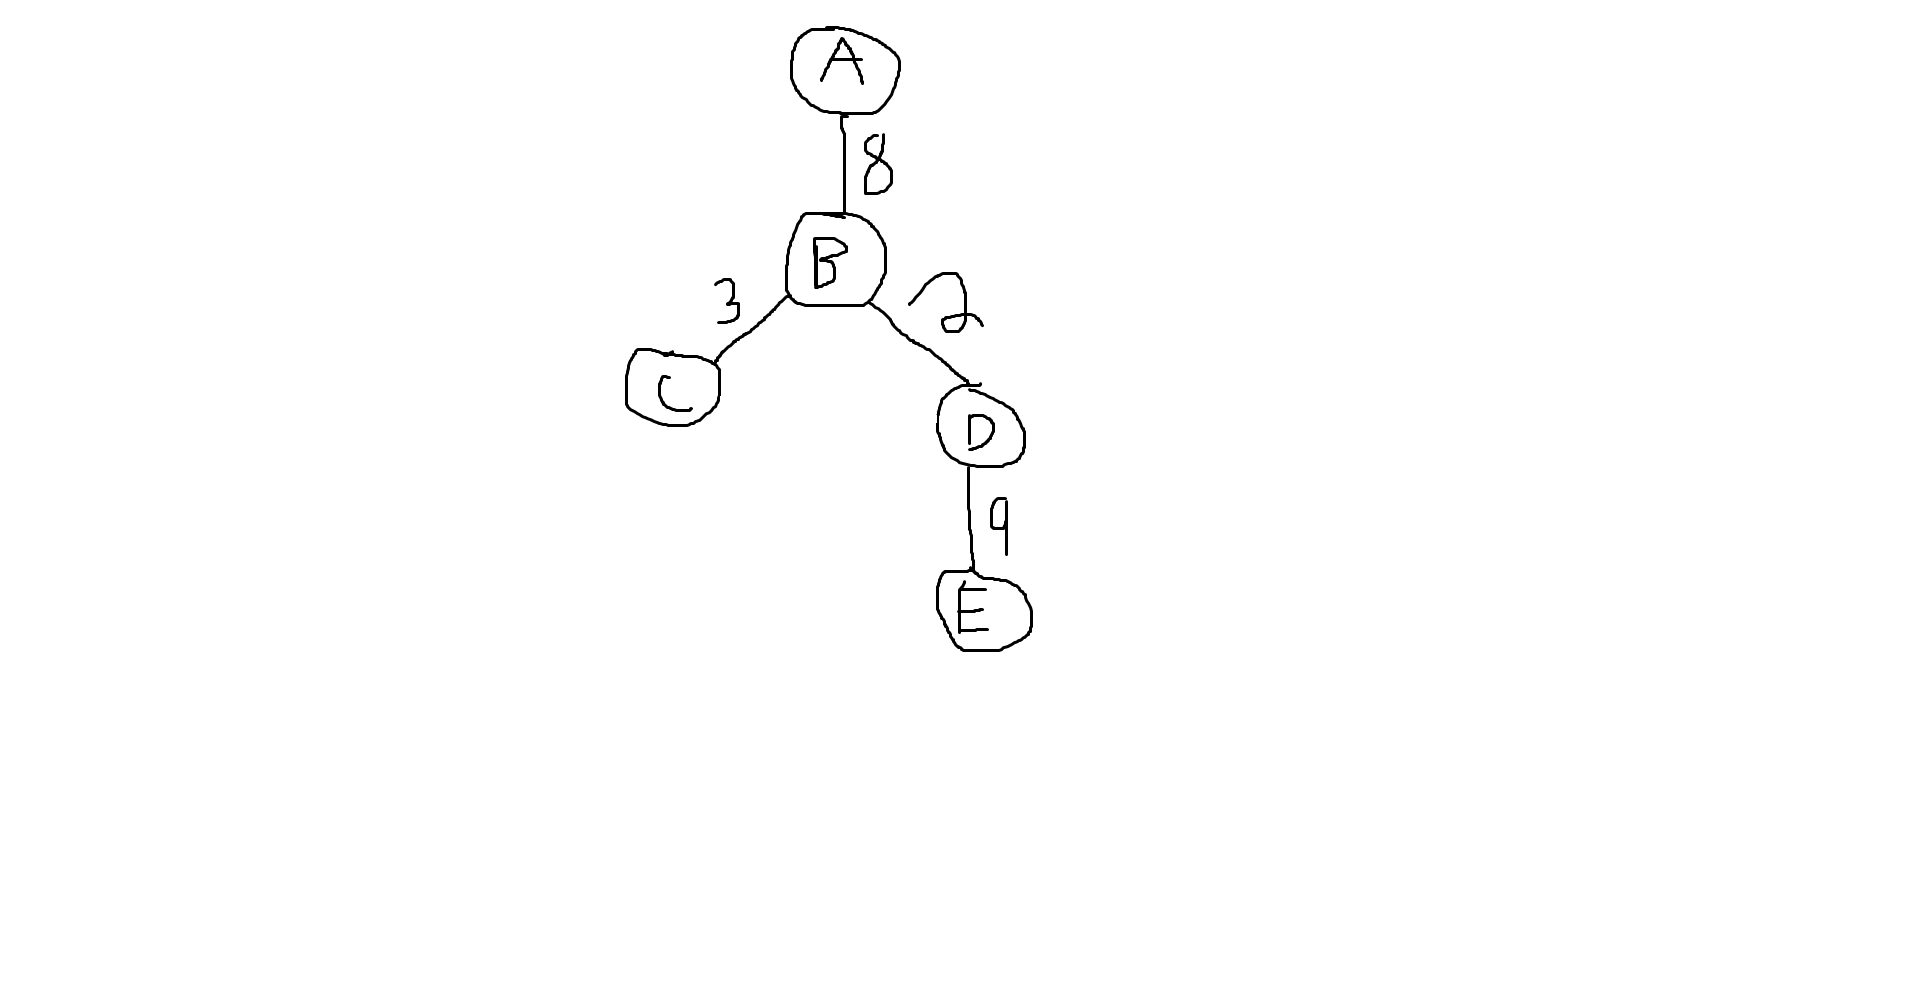
\includegraphics[scale=0.3]{MLT2} \newline$ This is a minimum limiting tree, since all trees in this graph must necessarily be a minimum limiting tree. However, since the smallest edge has been removed, it cannot be a minimum spanning tree. $\newline \newline$ Therefore, by contradiction, all MLT are not necessarily MST.
\end{solution}

\pagebreak
\item (7 pts) Prove that every MST of $G$ is a minimum-limiting tree of $G$. [\textbf{Hint:} Let $T$ be an MST of $G$, and let $T^{\prime}$ be a minimum-limiting tree of $G$. If $T$ is not a minimum-limiting tree, can we replace the heaviest edge of $T$? Think about how to use $T^{\prime}$ here.]

%Is every MST of $G$ a minimum-limiting tree of $G$? Prove or give a counterexample.
\begin{solution}
Say, within our tree T, we have our largest edge E. Let us say this is a larger edge than the minimum limiting edge from T`, E`, such that E $\geq$ E`. $\newline \newline$ Since E is larger than E`, we should try and replace value E for an E to make E=E`. By the nature of a MST, however, any edge replacement in the graph for this edge will be a higher value than this edge, as otherwise this spanning tree will not be a minimum spanning tree. With no lower edges to come by and E being the highest in our minimum tree, E fits the definition of a limiting edge. Thus, E cannot be higher than E`, as otherwise it will not fit the definition of a MST. E cannot be lower than E`, as that would go against the definition of a limiting edge and make E` not a limiting edge. $\newline \newline$ Therefore, E must equal E` and the MST must also be an MLT for all limiting edges E.
\end{solution}

\end{enumerate}

\end{enumerate}

\pagebreak
\textbf{Ungraded questions} - These questions are for your practice. We won't grade them or provide a typed solution but we are open to discuss these in our OHs and you should take feed backs on your approach during the OHs. These questions are part of the syllabus. 

\begin{enumerate}

\item Suppose you are given the minimum spanning tree $T$ of a given graph G (with $n$ vertices and $m$ edges) and a new edge $e=(u,v)$ of weight $w$ that will be added to $G$. Give an efficient algorithm to find the MST of the graph $G\cup e$, and prove its correctness. Your algorithm should run in $O(n)$ time.\\
\begin{solution}

\end{solution}

\item Based on the following graph :
\begin{figure}[h!]
\begin{center}
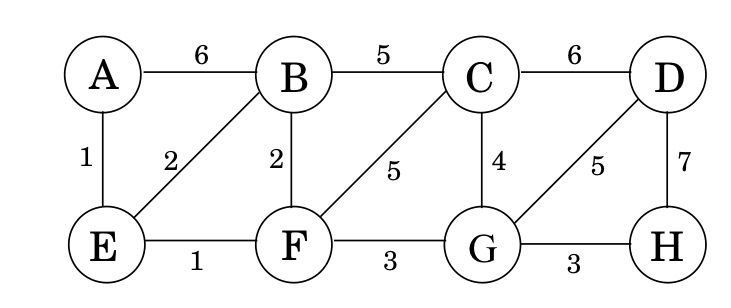
\includegraphics[scale=0.3]{mst_graph_q2.jpg} 
\end{center}
\end{figure}

\begin{enumerate}[label=(\alph*)]

\item Run Kruskal's and find the MST. You can break the ties however you want. Draw the MST that you found and also find it's total weight.
\begin{solution}

\end{solution}
\pagebreak
\item Run Prim's starting from vertex $A$ and find the MST. You can break the ties however you want. Draw the MST that you found and also find it's total weight. Is the total weight same as what you get from the above?
\begin{solution}

\end{solution}
 
\end{enumerate}

\item Consider the following unweighted graph, and assign the edge weights (using positive integer weights only), such that the following conditions are true regarding minimum spanning trees (MST) and single-source shortest path (SSSP) trees:
	\begin{itemize}
	\itemsep-0.1pt
	\item The MST is distinct from any of the seven SSSP trees.
	\item The order in which Prim's algorithm adds the safe edges is different from the order in which Kruskal's algorithm adds them.
	\end{itemize}
	Justify your solution by (i) giving the edges weights, (ii) showing the corresponding MST and all the SSSP trees, and (iii) giving the order in which edges are added by each of the three algorithms. 	
	\begin{figure}[h!]
\begin{center}
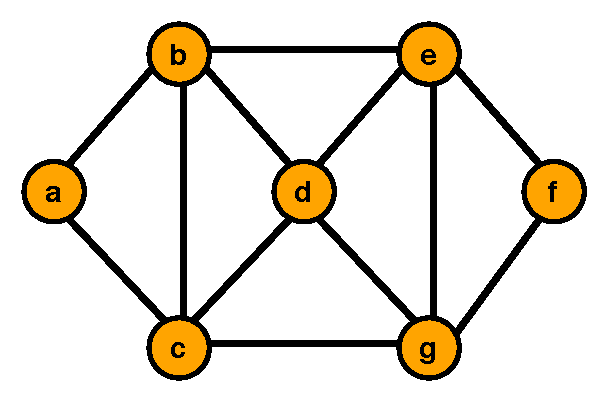
\includegraphics[scale=0.6]{graph_mst.pdf} 
\end{center}
\end{figure}

\begin{solution}

\end{solution}

\end{enumerate}

\end{document}
